

% From Master's thesis:
The SM is a collection of relativistic quantum field theories (QFT) that describe the interactions between all known fundamental particles.
% It has been extremely successful in describing correctly an enormous amount of experimental measurements. 
% The latest achievement is the discovery of the Higgs boson in 2012.
% It has been extremely successful in making predictions that were later confirmed by experimental measurements. 
% Examples are the observation of the $W$ and $Z$ bosons in 1983 by the UA1 and UA2 collaborations, or the top quark discovery in 1995 by the CDF and D0 experiments. \todo{Maybe references}
% The success story culminated in the discovery of a new particle by the ATLAS and CMS collaborations in 2012~\cite{HIGG-2012-27,CMS-HIG-12-028}.
% The observation of the $W$ and $Z$ bosons by the UA1 and UA2 collaborations in 1983 are just two examples of this.
% The discovery of the long sought-after Higgs boson in 2012 by the ATLAS and CMS collaborations~\cite{Aad:2012tfa,Chatrchyan:2012xdj} marks the highlight of this success story. 
%The success story culminated in the discovery of a new particle by the ATLAS and CMS collaborations in 2012~\cite{HIGG-2012-27,CMS-HIG-12-028}. 
% To date, ten years after this discovery, all experimental measurements show consistency of the observed particle with the properties of the long sought-after Higgs boson predicted by the SM.
The fundamental particles (also called \emph{elementary particles}) are grouped according to their quantum numbers, and their interactions are described by the requirement of local gauge invariance with respect to the gauge group
\begin{equation}
  \label{eq:sm-gauge-group}
  \text{SU(3)}_C \times \text{SU(2)}_L \times \text{U(1)}_Y,
\end{equation}
the details of which are explained in this section.
% The mathematical formulation SU(3)$_C$ $\times$ SU(2)$_L$ $\times$ U(1)$_Y$ local gauge symmetry that gives rise to the interactions between all known fundamental particles.
%It evolved during the 60’s and 70’s due to a strong interplay between experimental observations and theoretical developments. 
\Cref{subsec:particle-content} provides a high-level overview of the particles and forces that are part of the SM. \Cref{subsec:formalism} briefly outlines the theoretical principles that build the basis for the mathematical description of the SM. The remaining sections summarize the Lagrange formulation of the SM.
%, focusing on the \emph{Higgs mechanism} of \emph{electroweak symmetry breaking} (EWSB).
% \Cref{subsec:qed,subsec:qcd,subsec:ew-model,subsec:ewsymbreaking,subsec:fermion-masses,subsec:final-lagrangian} summarize the mathematical formulation of the SM, focusing on the \emph{Higgs mechanism} of \emph{electroweak symmetry breaking} (EWSB).
% The free parameters of the SM are summarized in \cref{subsec:final-lagrangian}, and \cref{sec:limitations} concludes this section by discussing the limitations of the SM.
% that motivate conducting more precise measurements such as the one presented in \cref{chap:hww} of this thesis.
The SM is covered in all its detail in the literature, e.g. \ccite{Peskin:1995ev,Halzen:1984mc,Thomson:2013zua}, which serve as the primary resources for the descriptions in this section.


% From previous theoretical foundation intro:
% - Section underlines the theoretical underpinnings that manifest the Higgs boson as a special place in the universe
% - Lots of SM parameters are related to Higgs (SM stands and falls with Higgs)
% - The SM also has limitations -> precision measurements of Higgs required
% - Many models of new physics expect to have access to new physics through interactions with Higgs ()


%On a phenomenological level, fundamental physics can be described in terms of elementary particles and forces. 
% - Introduction to QFT and gauge group
% - Lagrangian formalism
% - local gauge invariance: without local gauge invariance:

% From Pich The Standard Model
% Thus, once a given phase convention has been adopted at one reference point x0, the same convention must be taken at all space-time points. This looks very unnatural.

% - highly successful in describing QED
% WHAT HAPPENS IN THIS SECTiION:

% - First overview of particles and forces
% - Formalism
% - QED, QCD, electroweak model
% - Problem: no masses for bosons -> Higgs mechanism
% - Final Lagrangian and parameters to be measured experimentally of the SM
% - Limitations of the SM

\subsection{Particles and forces}
\label{subsec:particle-content}
%In QFT all fundamental fields have an associated particle, that can be thought of as excitations (or vibrations) of the fields.
QFT describes nature in terms of fundamental fields and their interactions. Each field is associated with an elementary particle that can be thought of as a quantum excitation of the underlying field.
This association makes it possible to describe fundamental physics using elementary particles.
%\footnote{To simplify terminology, the objects are mostly referred to as particles rather than fields in this chapter, but the relationship is important to be kept in mind.} 
% On a \TDnote{phenomenological}{other word?} level, fundamental physics can be described in terms of elementary particles and forces.
% All currently known particles and forces included in the SM are listed in \TDnote{REF}{REF}.
The particle content of the SM is summarized in \cref{fig:particles-infographic}.
The particles can be grouped into two main types:
\emph{fermions} with half-integer spin and \emph{bosons} with integer spin. The interaction between the fermions (sometimes called \emph{matter particles}) are interpreted as exchanges of \emph{gauge bosons} (also called \emph{force carriers}) that mediate the fundamental forces.
% \emph{fermions} with half-integer spin (sometimes called \emph{matter particles}) and \emph{bosons} with integer spin (known as the \emph{mediators} or \emph{force carriers} of the fundamental forces).

The fermions can be grouped into three generations, each containing two leptons and two quarks. The different types of leptons and quarks are referred to as (quark or lepton) \emph{flavors}. The fermions can be categorized in terms of their mass and quantum numbers such as \emph{charge} and \emph{hypercharge}. Quarks have an additional property called \emph{color}, which can take three possible values typically labelled as red, green, and blue\footnote{In fact, also linear combinations of the three colors are realized in nature, as discussed later in this chapter.}.
Additionally, each fermion has a corresponding antiparticle that has the same mass but ``opposite'' internal quantum numbers, i.e., oppositely signed charge and anti-color if applicable.
\begin{figure}[ht]
  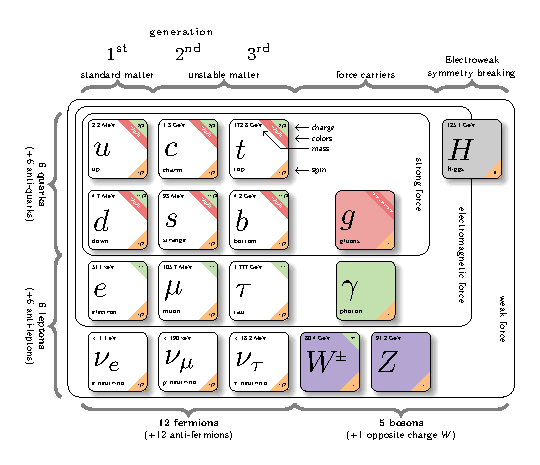
\includegraphics[width=1\textwidth,trim=10 0 10 0]{figures/theory/particles-infographic/particles-infographic.pdf}
  \caption[Overview of particles in the SM.]{Overview of the particles in the SM. Their charge, color, mass, and spin are indicated. More details are given in the text. The graphic is adapted from \ccite{CBurgardParticlesInfographic} and the values taken from \ccite{PDG2020}.}
  \label{fig:particles-infographic}
\end{figure}

%The interactions between the fermions can be described by exchanges of so-called \emph{gauge bosons}.
The SM includes three of the four known fundamental interactions: The \emph{electromagnetic interaction}, the \emph{strong interaction}, and the \emph{weak interaction}. The electromagnetic and the weak interactions are unified in the \emph{electroweak theory}. The fourth known fundamental interaction, \emph{gravitation}, is not part of the SM but can be fully neglected in present particle physics experiments due to its weak strength.

The gauge boson that mediates the electromagnetic interaction is the massless \emph{photon} that interacts with all charged particles. Electromagnetic interactions are described by the theory of \emph{quantum electrodynamics} (QED). The strong interaction is transmitted via eight massless gluons, following the rules of \emph{quantum chromodynamics} (QCD). QCD acts on matter particles that carry color, that is, quarks and gluons themselves.
Due to a property known as \emph{confinement} in QCD\footnote{Confinement arises due to the energy dependence of the strength of the QCD interactions (see \cref{subsec:factorisation}).}, quarks cannot be found in isolation. They are confined within hadrons that consist, for example, of a quark and an anti-quark (known as \emph{mesons}) or three quarks (known as \emph{baryons}).
The weak interaction is mediated by three massive gauge bosons, \Wplus, \Wminus, and \Zboson, and acts on all fermions. Similar to gluons, the \Wpm and \Zboson bosons can interact with themselves.

The final particle of the SM is the electrically neutral \emph{Higgs boson}. It is the only spin-0 scalar particle and plays a special role in the SM in the mechanism of electroweak symmetry breaking through which the \Wpm and \Zboson bosons gain their masses. A dedicated overview of the physics involving the Higgs boson is provided in \cref{chap:higgs}.


\subsection{Formalism and principles}
\label{subsec:formalism}
% - Action: S = Int ( Lagrangian ) dt -> EOMs
% - Lagrangian = Int (Lagrange density ) d3x
% -> Lagrange density is commonly referred to as Lagrangian 
% - In QFT, we define EOMs for fields by specifying the Lagrange density (Lagrangian)

% ONE MORE SENTENCE:
% In physics, equations of motion are equations that describe the behavior of a physical system in terms of its motion as a function of time.[1] More specifically, the equations of motion describe the behavior of a physical system as a set of mathematical functions in terms of dynamic variables.

% Particles can be thought of as excitations (or vibrations) of corresponding fundamental fields. 
In order to describe the behavior of a physical system, the equations of motions can be derived from Lagrange's equations
\begin{equation}
  \label{eq:euler-lagrange}
  \frac{\partial}{\partial x} \left( \frac{\partial \Lagrangian}{\partial \left(\partial \psi / \partial x \right) } \right) - \frac{\partial \Lagrangian}{\partial \psi} = 0,
  %S = \int \Lagrangian d^3x dt,
\end{equation}
where \Lagrangian is the Lagrange density and $\psi$ is a particle field.\footnote{Details on the Lagrange formalism can be found in any standard textbook on QFT, e.g. in \ccite{Peskin:1995ev}.}
The dynamics of a system are therefore fully specified by the Lagrange density, often simply denoted \emph{Lagrangian}.
The Lagrangian is generally a function of the fields $\psi$, their derivatives $\partial \psi = \frac{\partial \Lagrangian}{\partial x}$, and the space-time coordinate $x$, so $\Lagrangian \to \Lagrangian \left( \psi, \partial \psi, x \right)$.
The fields are generally dependent on the space-time coordinate, $\psi \rightarrow \psi(x)$.\footnote{For cleaner notation, these dependencies are not explicitly mentioned throughout this thesis.}

For a given field $\psi$, the principles of QFT demand to include all possible interaction terms in the Lagrangian that are related to the field\footnote{This follows what is sometimes referred to as the ``totalitarian principle'' of quantum mechanics, that satirically states: ``Everything not forbidden is compulsory'', meaning that everything allowed by the laws of physics must actually happen or exist.}.
The number and type of terms that can be included in the SM, however, is strongly constrained by requiring the theory to be invariant under symmetry transformations of the fields following the SM gauge group shown in \cref{eq:sm-gauge-group}.
The SM is governed by the principle of \emph{local gauge invariance}, which implies that the physical content of the theory stays the same when performing transformations of the particle fields according to
\begin{equation}
  \psi \rightarrow e^{iT(x)} \psi
\end{equation}
independently at every space-time point, where $T(x)$ is the generator of a certain symmetry group.
% Gauge theories require the introduction of so-called gauge fields, that transform in a way so that the theory stays locally gauge invariant.
% Pich
% This is only possible if one adds an extra piece to the Lagrangian, transforming in such a way as to cancel the ∂μθ term in Eq. (6).
% In order to maintain the symmetry, the Lagrangian may need to be manipulated by introducing new fields.
Local gauge theories require the introduction of \emph{covariant derivates} to make the Lagrangian invariant under local gauge transformations. These covariant derivatives include gauge fields which give rise to particle interactions identified as the fundamental forces of nature.
Historically, QED is the first local gauge theory that was established. It follows a U(1) local gauge symmetry and entails the photon as the associated gauge field.
The SM can be elegantly described by demanding local gauge invariance with the symmetry group as shown in \cref{eq:sm-gauge-group}, and explains the existence of all gauge bosons mentioned in the previous section.
The fermions, in contrast, are added a priori to the theory and do not follow from fundamental principles.
%The following sections provide an overview of the Lagrangian of the SM, by going through the different symmetry groups. 
The following sections will outline the Lagrange formulation of the SM.
In all equations, natural units are used, i.e. $c = \hbar = 1$, which leads to the mass, momentum, and energy of particles being expressed in units of electronvolt (\eV).
Moreover, the Einstein-summation convention is used and if not mentioned otherwise, greek-letter indices take integer values from 1 to 4, while latin-character indices take integer values from 1 to 3.

% - renormalization:
% We consider that the physics is understood up to a given cut-off/scale Lambda.

%The SM is governed by the principle of local gauge invariance and the associated symmetry group is SU(3)$_C$ $\times$ SU(2)$_L$ $\times$ U(1)$_Y$. 

% the next important lesson is that the existence of these symmetries places suck an incredibly strong constraint on what the theory actually is.

% Sean
% QED: demanding all the terms in your Lagrangian being gauge invariant is enforcing the conservation of electric charge gauge
% This is a reflection of Noethers theory. Symmetry conservation -> associated quantity of the U(1) symmetry is charge

% Sean Carrol:
% W and Z bosons are the physical excitations from vibrations in the SU(2) to gauge field
%the existence of these fields giving rise to interactions giving rise to forces of nature comes from the gauge symmetry.
% the next important lesson is that the existence of these symmetries places suck an incredibly strong constraint on what the theory actually is.

% From Master thesis
% An essential part of the mathematical formulation of the SM is based on the postulation of local gauge invariance. It implies, that the physical content of the theory should stay the same when performing certain redefinitions of the particle fields independently at every space-time point. The SM follows a SU(3)×SU(2)L×U(1)Y symmetry group, where SU(3) is the gauge group of QCD and SU(2)L×U(1)Y the corresponding symmetry for the electroweak model (the meaning of the subindizes L and Y will be explained in the following sections). Historically, QED was the first well established gauge theory, following a U(1) symmetry. To demonstrate the principles of a gauge theory, which are the key concepts of the mathematical framework of the SM, the QED Lagrangian will be derived in the following. Subsequently the same principles are applied to describe the main aspects of the more complex theories of QCD and the electroweak model. A description of the mechanism to incorporate masses for the W± and Z bosons via breaking the electroweak symmetry is given thereafter. The following sections follow to a large extend the more detailed descriptions given in Refs. [19–21].


\subsection{Quantum electrodynamics}
\label{subsec:qed}
%The above derivations are shortly recapped: Starting from the Lagrangian of a freely moving relativistic fermion one can impose the requirement of local U(1) gauge invariance. This demands to add a new field $A_\mu$ toghether with an interaction term, which is incorporated in the Lagrangian by introducing a covariant derivative $D_\mu$. Additionally, the kinetic term in \cref{eq:kinetictermqed} needs to be added for the new field, which leads to the final Lagrangian for QED, shown in \cref{eq:Lagrangianqed}.
QED can be regarded as a reflection of an underlying $U(1)$ local gauge symmetry of the complex-valued fermion fields, $\psi_f$, known as \emph{Dirac spinors}.
The Lagrangian that is invariant under $\psi_f \rightarrow e^{i \omega(x)} \psi_f$ transformations can be written as
\begin{equation}
  \mathcal{L}_{\text{QED}} = \sum_f \bar{\psi}_f(i\gamma^\mu D_\mu - m_f)\psi_f - \frac{1}{4}F_{\mu\nu}F^{\mu\nu},
  \label{eq:Lagrangianqed}
\end{equation}
where the sum goes over all electrically charged fermions with masses $m_f$, and $\gamma^\mu$ refers to the four $4 \times 4$ gamma matrices.
Here, $D_\mu = \partial_\mu + ieA_\mu$ is the covariant derivative, which includes the gauge field $A_\mu$ which is associated with the photon. The requirement of local gauge symmetry prohibits terms quadratic in $A_\mu$, resulting in the prediction of the photon being massless.\footnote{Masses of a certain field arise from terms in the Lagrangian that are quadratic in that field.}
The so-called \emph{field tensor}, defined as $F_{\mu\nu} = \partial_\mu A_\nu - \partial_\nu A_\mu$, provides an elegant mathematical object representing the electromagnetic field. It can be used, for example, to describe Maxwell's equations of classical electrodynamics.

The symmetry group associated to QED is denoted U(1)$_{\text{QED}}$ and the conserved quantity is the electric charge.\footnote{This is a reflection of Noether's theorem, which states that each symmetry is related to a conserved quantity.}
It should be noted that U(1)$_{\text{QED}}$ is not part of the original symmetry group of the SM. As explained below, U(1)$_{\text{QED}}$ arises from a SU(2)$_L$ $\times$ U(1)$_Y$ symmetry that is spontaneously broken.


\subsection{Quantum chromodynamics}
\label{subsec:qcd}
QCD is a non-Abelian gauge theory associated to a SU(3)$_C$ symmetry. The subindex $C$ refers to the color which is the conserved quantity under SU(3)$_C$ transformations.
The locally gauge invariant QCD Lagrangian reads
\begin{equation}
  %  \mathcal{L}_{\text{QCD}} = -\frac{1}{4}G_{\mu\nu}^aG^{a\,\mu\nu} + \bar{q}^i\left( i\gamma^\mu D_\mu-m \right)^j_i q_j,
  \mathcal{L}_{\text{QCD}} = \sum_f \bar{\psi}_f(i\gamma^\mu D_\mu - m_f)\psi_f - \frac{1}{4}G_{\mu\nu}^aG^{\mu\nu}_{a},  \label{eq:lqcd}
\end{equation}
where the sum runs over all quark fields, $\psi_f$, that take the form of spinor triplets.
%\todo{Sum over A in lambdaA GmuA in the equation?} <- YEP! Because of self interaction
The covariant derivate is given by
\begin{equation}
  D_\mu = \partial_\mu + i g_s \frac{\lambda^a}{2} G_\mu^a,
\end{equation}
which includes eight gluon fields $G_\mu^a$ (with $a = 1, \ldots, 8$), the strong coupling constant $g_s$, and the Gell-Mann matrices $\lambda^a$ that are the generators of the SU(3)$_C$ group.
The field tensors $G_{\mu\nu}^a$ are defined as
\begin{equation}
  \label{eq:qcd-tensor}
  G_{\mu\nu}^a = \partial_\mu G_\nu^a - \partial_\nu G_\mu^a - g_s f^{abc}G_\mu^b G_\nu^c,
\end{equation}
where $f^{abc}$ are the structure constants of SU(3)$_C$, with $a, b, c = 1, \ldots, 8$.
The term involving $f^{abc}$ includes an implicit sum over similar latin-character indices. It arises from the non-commuting elements of the SU(3)$_C$ group and gives rise to triple and quartic gluon self-interactions, which separates QCD from QED.
% Triple and quartic self-interactions are part of QCD because gluons themselves carry a combination of a color and anti-color. 
% Invariant under ... transformation, where ... are the group generators
Similar to photons, the gluons are massless because no terms quadratic in the gluon fields are allowed because of the requirement of local gauge invariance.
%which is similar to the requirement of a massless photon in QED. 



\subsection{The electroweak model}
\label{subsec:ew-model}
% - the chirality can be determined with... right-chiral fermions are singlets under SU(2)L transformations
% - This also means that no right-chiral neutrinos exist in the SM as they don't interact with any of the forces

% "Also called: The Glashow􏰁Weinb erg􏰁Salam Theory of Weak Interactions"
The weak and electromagnetic forces are unified in the electroweak model~\cite{GLASHOW1961579,SALAM1964168,PhysRevLett.19.1264} by imposing local gauge invariance under transformations of the symmetry group
\begin{equation}
  \label{eq:ew-sym-group}
  \text{SU(2)}_L \times \text{U(1)}_Y.
\end{equation}
The electroweak gauge group is based on two major empirical findings.
The first is, that only \emph{left-chiral}\footnote{
  The \emph{chirality} of a fermion can be determined with the projection operators $P_L$ and $P_R$ like \\
  $\psi = P_L \psi + P_R \psi = \frac{1}{2} \left( 1 - \gamma^5 \right) \psi + \frac{1}{2} \left( 1 + \gamma^5 \right) \psi = \psi_R + \psi_L$, \\
  where $\gamma^5 = i\gamma^0\gamma^1\gamma^2\gamma^3$. The chirality becomes identical to the helicity for massless particles.} (also denoted \emph{left-handed}) fermions interact via the weak interaction, indicated with an $L$ in \cref{eq:ew-sym-group}. An overview of the fermion content is shown in \cref{tab:ewfermioncontent}, that groups the fermions into left-handed doublets, $\psi_L$, and right-handed singlets, $\psi_R$, under SU(2)$_L$ transformations.
The second finding is that the quarks participating in the electroweak interaction, labelled as $u', d', c'$, are a mixture of the quark mass eigenstates. Their relation is specified by the \emph{Cabibbo–Kobayashi–Maskawa (CKM) matrix} \cite{doi:10.1143/PTP.49.652}, $\pmb{V}$, as
% From Peskin
% The off diagonal terms in Vij allow weak􏲩interaction transitions b e􏲩 tween quark generations.
\begin{equation}
  \begin{pmatrix}
    d' \\
    s' \\
    b'
  \end{pmatrix}
  =
  \pmb{V}
  \begin{pmatrix}
    d \\
    s \\
    b
  \end{pmatrix}.
\end{equation}
The CKM matrix is unitary and fully specified with 4 parameters and encodes the strength of the flavor-changing electroweak interactions.
%\todo{Maybe add one more sentence describing the rotation that is necessary? see P.Sommer thesis}

The fermion fields then transform as
\begin{align}
  \psi_L & \rightarrow e^{iY\omega} e^{iT^a\omega_a} \psi_L, \qquad (a = 1, 2, 3) \\
  \psi_R & \rightarrow e^{iY\omega} \psi_R,
\end{align}
under SU(2)$_L$ $\times$ U(1)$_Y$ transformations, where $T^a=\frac{\sigma^a}{2}$ are the Pauli matrices and generators of the SU(2)$_L$ group.
The associated conserved quantity is the \emph{weak isospin} $T$, of which the third component is conserved in weak interactions and given by $T^{(3)} = \pm \frac{1}{2}$ for SU(2)$_L$ doublets and $T^{(3)} = 0$ for SU(2)$_L$ singlets.
The U(1)$_Y$ symmetry is associated to the \emph{hypercharge} $Y$, and cannot be directly associated to the QED gauge group.
The relation to the electromagnetic interaction and the physical electric charge $Q$ is
\begin{equation}
  Q = T^{(3)} + \frac{Y}{2}.
\end{equation}

\noindent The local gauge invariant electroweak Lagrangian can be written as
\begin{equation}
  \mathcal{L}_{\text{EWK}} = \sum_f i\bar{\psi}_{f}\gamma^\mu D_\mu \psi_{f} - \frac{1}{4}W_{\mu\nu}^aW^{\mu\nu}_{a} - \frac{1}{4} B_{\mu\nu}B^{\mu\nu},
  \label{eq:lagrangianewk}
\end{equation}
where the sum runs over all fermions $f$, including their left-handed and right-handed counterparts.
%, whose occurrence as left-handed and right-handed particles is explicitly mentioned.
The covariant derivative is defined as
\begin{equation}
  D_\mu = \partial_\mu + igT^aW_\mu^a + ig'\frac{Y}{2}B_\mu
  \label{eq:covdevewk}
\end{equation}
and includes four gauge fields. The fields $W^a_\mu$ (with a = 1, 2, 3) are the gauge fields of SU(2)$_L$ with associated coupling $g$, and $B_\mu$ is the gauge field of U(1)$_Y$ with coupling $g'$.
The field tensors in \cref{eq:lagrangianewk} are given by
\begin{align}
  W_{\mu\nu}^a & = \partial_\mu W_\nu^a - \partial_\nu W_\mu^a - g \epsilon^{abc} W^b_\mu W^c_\nu, \label{eq:Wtensor} \\
  B_{\mu\nu}   & = \partial_\mu B_\nu - \partial_\nu B_\mu,
\end{align}
where $\epsilon^{abc}$ are the structure constants of SU(2)$_L$. The third term on the right-hand side of \cref{eq:Wtensor} includes an implicit sum over similar latin-character indices. It arises because of the non-Abelian nature of SU(2)$_L$ and gives rise to triple and quartic self-interactions of the gauge fields $W_{\mu}^a$.
The tensor $B_{\mu\nu}$ has the same structure as the electromagnetic field strength tensor obtained in QED.
%\TDinote{}{Give details on structure constants? for QCD AND Electroweak model}

\noindent The Lagrangian of \cref{eq:lagrangianewk} describes 4 massless bosons. No terms quadratic in the vector fields are allowed due to the requirement of local gauge invariance.
Another mechanism is required to explain the existence of the masses of the gauge fields \Wpm and \Zboson.
% and $\gamma$. 

  \begin{table}
    \caption[Overview of the fermion content in the electroweak model.]{Overview of the fermion content in the electroweak model with the quantum numbers of the weak isospin $T^3$, hypercharge $Y$ and electric charge $Q$. They are grouped into left-handed doublets and right-handed singlets denoted with the subindex $L$ and $R$ respectively. The down-type quarks $d', s', b'$ are the eigenstates of the electroweak interaction and given by linear combinations of the mass eigenstates $d, s, b$. This mixing is described by the CKM matrix, see text. Since right-handed neutrinos are not undergoing any interaction they do not play a role in the Standard Model and are not listed here.}
    \label{tab:ewfermioncontent}
    \centering
      \begin{tabular}{c |@{}| c c c | c c c}
        \toprule
                                 & \multicolumn{3}{c}{Generation}          & \multicolumn{3}{|c}{Quantum number}                                                                                                            \\
                                 & 1$^{\text{st}}$                         & 2$^{\text{nd}}$                             & 3$^{\text{rd}}$                               & $T^3$          & $Y$            & $Q$            \\
        \midrule
        \multirow{3}{*}{Leptons} & \multirow{2}{*}{$\myvec{\nu_e                                                                                                                                                            \\ e}_L$} & \multirow{2}{*}{$\myvec{\nu_\mu \\ \mu}_L$} & \multirow{2}{*}{$\myvec{\nu_\tau \\ \tau}_L$} & $\frac{1}{2}$  & -1             & 0 \\
                                 &                                         &                                             &                                               & $-\frac{1}{2}$ & -1             & -1             \\
                                 & $e_R$                                   & $\mu_R$                                     & $\tau_R$                                      & 0              & -2             & -1             \\
        \midrule
        \multirow{3}{*}{Quarks}  & \multirow{2}{*}{$\myvec{u                                                                                                                                                                \\ d'}_L$}    & \multirow{2}{*}{$\myvec{c \\ s'}_L$}        & \multirow{2}{*}{$\myvec{t \\ b'}_L$}          & $\frac{1}{2}$  & $\frac{1}{3}$  & $\frac{2}{3}$ \\
                                 &                                         &                                             &                                               & $-\frac{1}{2}$ & $\frac{1}{3}$  & $-\frac{1}{3}$ \\
                                 & $u_R$                                   & $ c_R$                                      & $t_R$                                         & 0              & $\frac{4}{3}$  & $\frac{2}{3}$  \\
                                 & $d_R$                                   & $ s_R$                                      & $b_R$                                         & 0              & $-\frac{2}{3}$ & -$\frac{1}{3}$ \\
        \bottomrule
      \end{tabular}
  \end{table}




% From experiments one expects two charged bosons $W^\pm$ and two neutral bosons, the $Z$ and the photon.

\subsection{Spontaneous symmetry breaking and the Higgs mechanism}
\label{subsec:ewsymbreaking}
%- Local gauge invariance does not allow adding mass terms
%- The SU(2)$_L$ $\times$ U(1)$_Y$ symmetry is spontaneously broken into U(1)$_\text{QED}$
%- This mechanism is spontaneous symmetry breaking
%- Simply put, the Lagrangian itself maintains the symmetry, but the state of lowest energy is not invariant and breaks the summetry.
% - Could add mass terms disregarding local gauge invariance but this would render theory unrenormalizable
%naturally appear in the Higgs mechanism explained below.
%An additional mechanism is needed in the SM to explain the finite masses of the weak gauge bosons. 

A principle known as \emph{spontaneous symmetry breaking}, that was first explored in the field of condensed-matter physics, can be used to generate mass terms for the weak gauge bosons without violating local gauge invariance.
This was first formulated in particle physics by three independent research teams in 1964: Brout and Englert~\cite{PhysRevLett.13.321}, Higgs~\cite{PhysRevLett.13.508,HIGGS1964132}, and Guralnik, Hagan, and Kibble \cite{PhysRevLett.13.585}. Their work was inspired by previous advancements in the theory of superconductivity~\cite{PhysRev.108.1175} and specifically P. W. Anderson, who proposed the mechanism of spontaneous symmetry breaking for generating mass terms in a non-relativistic scenario already in 1963~\cite{PhysRev.130.439}.
Today, the mechanism incorporated in the SM is most often called \emph{BEH mechanism} or \emph{electroweak symmetry breaking} (ESWB).
The basic principle is to allow the state of lowest energy to hide local gauge invariance while maintaining the gauge symmetry of the Lagrangian itself.

% From Peskin and Schroeder
% - In the theory of sup erconductiv􏰁 ity􏰔 for example􏰔 the Ab elian gauge invariance of electromagnetism is broken by pairs of electrons that condense in the ground state of a metal􏰎
%The mechanism is known as the \emph{Brout-Englert-Higgs mechanism} (or simply \emph{Higgs mechanism}) or also \emph{electroweak symmetry breaking} (ESWB).
%The underlying concept is that the Lagrangian itself maintains the symmetry, but the state of lowest energy is not invariant and breaks the gauge symmetry.
% was published almost simultaneously by three independent groups in 1964: by Robert Brout and François Englert;[3] by Peter Higgs;[4] and by Gerald Guralnik, C. R. Hagen, and Tom Kibble.[5][6][7]

The Higgs mechanism assumes a complex scalar field of the SU(2)$_L$ group,
\begin{equation}
  \phi = \frac{1}{\sqrt{2}} \myvec { \phi_1 + i \phi_2 \\ \phi_3 + i \phi_4},
\end{equation}
and introduces a potential of the form
\begin{equation}
  V(\phi) = \mu^2\phi^\dagger\phi + \lambda \left(\phi^\dagger\phi \right)^2.
  \label{eq:higgspotential}
\end{equation}
The Lagrangian
\begin{equation}
  \mathcal{L}_{\text{Higgs}} = |D_\mu\phi|^2 - V(\phi), % - \frac{1}{4} W_{\mu\nu}^a W^{a\, \mu\nu} - \frac{1}{4} B_{\mu\nu} B^{\mu\nu},
  \label{eq:lagrangianhiggs}
\end{equation}
where $D_\mu$ is defined as shown in \cref{eq:covdevewk}, is invariant under local SU(2)$_L$ $\times$ U(1)$_Y$ transformations.
The parameters of the potential $V(\phi)$ are specifically chosen to satisfy $\mu^2 < 0$ and $\lambda > 0$.
This choice provides the \emph{Higgs potential} with a characteristic shape, depicted in \cref{fig:higgspotential}, and gives rise to a set of degenerate ground state configurations satisfying
\begin{equation}
  |\phi| = \sqrt{ \frac{\mu^2}{2\lambda} } \equiv \frac{ v }{\sqrt{2}},
  \label{eq:higgsminima}
\end{equation}
where $v$ is the non-zero \emph{vacuum expectation value} (\emph{vev}) of the Higgs field.

\begin{figure}[t]
  \resizebox{0.75\textwidth}{!}{
    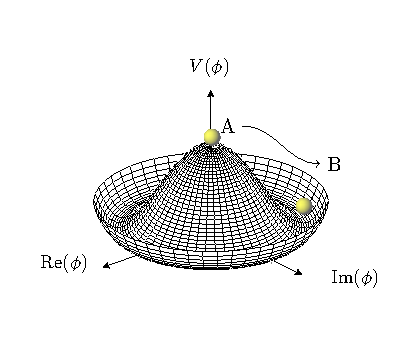
\includegraphics[trim=0 15 0 0]{figures/theory/higgs-potential/higgs-potential.pdf}
  }
  \caption[Illustration of the Higgs potential.]{Illustration of the Higgs potential $V(\phi)$ defined in \cref{eq:higgspotential} assuming a simplified Higgs field, a complex singlet scalar $\phi = \phi_1 + i \phi_2$. The minimum can be found on a circle in the $(\phi_1, \phi_2)$ plane.
  }
  \label{fig:higgspotential}
\end{figure}
%% We find that the Lagrangian for such a field
%% \begin{equation}
%% \end{equation}
%% is invariant under global SU(2) phase transformations
%It is invariant under gauge transformations but not the ground state, which can be found at
%The minimum of the potential can be found on the circle of minima where
%Once a ground state is chosen, the SU(2)$_L$ $\times$ U(1)$_Y$ symmetry becomes spontaneously broken.
% The symmetry is therefore spontaneously broken when a ground state is chosen. 
%The arbitrary choice of a ground state is said to spontaneously break the symmetry. 
Without loss of generality the ground state can be chosen to be
\begin{equation}
  \phi_0 = \frac{1}{\sqrt{2}} \myvec{0 \\ v},
  \label{eq:groundstate}
\end{equation}
i.e., $\phi_1 = \phi_2 = \phi_4 = 0$ and $\phi_3 = v$, which spontaneously breaks the SU(2)$_L$ $\times$ U(1)$_Y$ symmetry.
Expanding the field $\phi$ around the minimum to first order in the fields yields
\begin{equation}
  \phi(x) = e^{iT^a\frac{\phi_a(x)}{v}}\frac{1}{\sqrt{2}} \myvec{ 0 \\ v + h(x) },
  \label{eq:higgsexp}
\end{equation}
where the extra term $e^{iT^a\frac{\phi_a(x)}{v}}$ describes the fluctuations of the fields $\phi_1, \phi_2, \phi_4$ around the vacuum $\phi_0$.
These fields are known as the \emph{Goldstone bosons} and have no direct physical implications. They can be eliminated from the Lagrangian by choosing an appropriate gauge, the \emph{unitary gauge}, so that
\begin{equation}
  \phi(x) = \frac{1}{\sqrt{2}} \myvec{ 0 \\ v + h(x) }.
  \label{eq:expanded-groundstate}
\end{equation}
There remains only one real physical field, $h(x)$, which is called the \emph{Higgs field} and is associated with a neutral scalar boson, the \emph{Higgs boson}, labelled $H$.
The mass of the Higgs boson follows by inserting \cref{eq:expanded-groundstate} into \cref{eq:higgspotential},
\begin{equation}
  m_H = \sqrt{2} \mu = \sqrt{2 \lambda} v.
\end{equation}
Inserting \cref{eq:higgsexp} into \cref{eq:lagrangianhiggs} and using the relations
\begin{align}
  W_\mu^\pm & = \frac{1}{\sqrt{2}} \left( W_\mu^1 \mp iW_\mu^2 \right),  \quad \text{and} \\
  \myvec{Z_\mu                                                                            \\ A_\mu} &= \myvec{ \cos\theta_\text{w} \quad - \sin\theta_\text{w} \\ \cos\theta_\text{w} \quad -\sin\theta_\text{w} } \myvec{ W_\mu^3 \\ B_\mu},
\end{align}
where $\theta_\text{w}$ is the \emph{weak mixing angle} defined as $\sin\theta_\text{w}^2 = \frac{g'^2}{g^2+g'^2}$, leads to the following terms in the Lagrangian
\begin{equation}
  \mathcal{L}_m = \frac{1}{4} \left( v + H \right)^2  \left(g^2 W_\mu^+W^{-\,\mu} + \frac{g^2}{2\cos\theta_\text{w}^2} Z_\mu Z^\mu \right).
  \label{eq:lagrangianmasses}
\end{equation}
One can identify terms quadratic in the physical fields $\Wpm$ and $Z$, generated by the non-vanishing expectation value $v$, giving rise to the masses
\begin{align}
  m_W & = \frac{vg}{2},                     \\
  m_Z & = \frac{m_W}{\cos \theta_\text{w}},
  \label{eq:boson-masses}
\end{align}
of the weak gauge bosons.
The mass of the $W$ boson can be related to the Fermi constant, $G_F$, via $m_W = \frac{g}{4 * \sqrt{2}G_F}$.
No field quadratic in $A_\mu$ appears, which reflects the fact that the photon is massless.

% DIFFERENT Formulation: It is worth while to decompose the Lagrangian into its different pieces:
The Lagrangian in \cref{eq:lagrangianmasses} can be re-written after substituting the masses of the gauge bosons,
\begin{equation}
  \mathcal{L}_{\text{H,boson-coupling}} = m_W^2 W_\mu^+W^{-\,\mu} \left( \frac{2H}{v} + \frac{H^2}{v^2} \right) + \frac{1}{2} m_Z^2 Z_\mu Z^\mu \left( \frac{2H}{v} + \frac{H^2}{v^2} \right),
  \label{eq:higgsbosoncoupling}
\end{equation}
which predicts that the interaction between the Higgs boson and the massive gauge bosons is proportional to the square of the mass of the coupled bosons and involves triplet ($V^\dagger VH$) and quartic ($V^\dagger VHH$) couplings.

%and choosing a specific gauge (the unitary gauge) the field $\phi$ can be written as
% As shown below, introducing a complex SU(2)$_L$ doublet does not only give rise to the $\Wpm$ and $Z$ boson masses, but can also be used to construct mass terms for fermions. Hence, the Higgs field couples to all massive elementary particles.
% A more detailed descriptions on experimental Higgs boson physics and an overview of the current state of knowledge is given in \cref{sec:higgsphysics}.
% The parameters of the Higgs potential $\mu^2 = \lambda v^2$ can be fixed for one combination by measuring parameters of the electroweak theory, but the physical Higgs mass cannot be predicted. 
% Moreover, the last two terms in \cref{eq:higgsselfcoupling} predict that the Higgs field couples to itself with cubic and quartic interactions.
% The couplings of the Higgs boson to the weak gauge bosons are already expressed in \cref{eq:lagrangianmasses}.
%While the Higgs boson was discovered experimentally in 2012 \cite{Aad:2012tfa,Chatrchyan:2012xdj}, and is by now seen in several different production and decay modes, the Higgs boson self-couplings are still searched for.
% In summary, adding a complex scalar Higgs field to the electroweak model, together with a potential that exhibits a non-zero vacuum expectation value, provides the ingredients to obtain mass terms for the weak gauge bosons $W^\pm$ and $Z$ when choosing a ground state of the Higgs field which spontaneously breaks the symmetry.
% The three Goldstone bosons that arise can be eliminated from the Lagrangian by using its underlying local gauge symmetry. 
% This results in three bosons acquiring a mass and the appearance of one remaining scalar field $H$. 
% The photon remains massless, because the U(1)$_{\text{QED}}$ symmetry is unbroken. 

\subsection{Fermion masses}
\label{subsec:fermion-masses}
The previous section explained how the Higgs mechanism naturally gives rise to mass terms for the $\Wpm$ and $Z$ bosons.
%The finite fermion masses, however, do not directly follow and the simple inclusion of fermion mass terms is forbidden because they would violate SU(2)$_L$ gauge invariance.
% , given that a term
% \begin{equation}
%   -m_f \bar{\psi} \psi = -m_f \left( \bar{\psi}_R\psi_L + \bar{\psi}_L\psi_R \right)
%   \label{eq:fermionmassterm}
% \end{equation}
% because $\psi_L$ transforms as a doublet and $\psi_R$ as a singlet. 
The masses of the fermions can be explained with an ad-hoc solution by introducing interaction terms between the left-handed fermion fields and the Higgs field, both appearing as doublets under SU(2)$_L$ transformations.
%This is possible because both the left-handed fermions and the Higgs field appear as doublets under 
For leptons, only electrons, muons, taus, that appear in the lower part of the SU(2)$_L$ doublet (see \cref{tab:ewfermioncontent}), require mass terms, as neutrinos are assumed to be massless in the SM\footnote{See \cref{sec:limitations} for a brief discussion on neutrino masses.}.
For up-type quarks ($u$, $s$, and $t$ quark) to become massive, the fermion fields are coupled to the charge conjugate of the Higgs field,
\begin{equation}
  \phi^C = \frac{1}{\sqrt{2}} \myvec{v + h(x) \\ 0},
\end{equation}
after choosing a ground state similar to \cref{eq:expanded-groundstate}.
The interactions are known as \emph{Yukawa interactions} and can then be written in the form
\begin{equation}
  \mathcal{L}_\text{Yukawa} = - \sum_{i} Y_l^i \bar{\psi}^{i}_{L} \phi \psi^{i}_{R} - \sum_{ij} \left( Y_{\text{u-type}}^{ij} \bar{\psi}^{i}_{L} \phi \psi^{i}_{\text{u-type},R} + Y_{\text{d-type}}^{ij} \bar{\psi}^{i}_{L} \phi^C \psi^{j}_{\text{d-type}, R} \right) + \text{h.c.},
  \label{eq:lyukawa}
\end{equation}
where the first sum runs over all leptons, the second sum over all quarks, and h.c. stands for the Hermitian conjugate of the previous terms.
The left-handed fields are given as $\psi^{i}_{L}$ and include the three lepton- and quark doublets.
The right-handed lepton fields are labelled as $\psi_R^i$ and the quark fields as $\psi^{i}_{\text{u-type},L}$, $\psi^{i}_{\text{d-type},L}$.
The labels ``u-type'' and ``d-type'' refer, respectively, to the up-type quarks ($u$, $s$, $t$) and down-type quarks ($d$, $c$, $b$).
The \emph{Yukawa couplings} are labelled as $Y_l^i$ for leptons and as $Y_{\text{u-type}}^{ij}$ and $Y_{\text{d-type}}^{ij}$ for up-type and down-type quarks, respectively. The $Y_{\text{u-type}}^{ij}$ and $Y_{\text{d-type}}^{ij}$ are $3 \times 3$ matrices accounting for the fact that the eigenstates of the weakly interacting quarks do not correspond to their mass eigenstates.
%A rotation of the quark fields can be performed accounting for the mixing. 
% Mass terms for quarks can be added in a similar but slightly more involved way. The down-type quarks participating in the electroweak interaction (denoted $d'$, $s'$, $b'$) are a mixture of the quark mass eigenstates (denoted $d$, $s$, $b$). 
% For each quark doublet there are two mass terms generated. For lepton doublets only one mass term is added because right-handed neutrinos are not part of the SM. Assuming only one generation of fermions, with quarks $u$ and $d$ and leptons $e$ and $\nu_e$, the Yukawa term can therefore be written as
% \begin{equation}
%   \mathcal{L}_\text{Yukawa} = - Y_{ud} \bar{\psi}_{ud,L} \phi \psi_{u,R} - Y_{ud} \bar{\psi}_{ud,L} \phi \psi_{d,R} - Y_l \bar{\psi}_{e\nu_e,L} \phi \psi_{e,R} + \text{h.c.},
%   \label{eq:lyukawa}
% \end{equation}
% where $\psi_{l}$ stands for lepton fields and $\psi_{q}$ for the quark fields.

The mass terms appear from \cref{eq:lyukawa} once a ground state of $\phi$ is chosen and the Yukawa terms have been diagonalized, resulting in nine independent parameters $Y_f$.
They take the form
\begin{equation}
  m_f = \frac{Y_f v}{\sqrt{2}},
\end{equation}
which predicts that the coupling strength between the fermions and the Higgs field is proportional to the mass of the fermions.

%\subsection{Renormalization}
% From modern particle physics book
% As shown by ‘t Hooft, only theories with local gauge invariance are renormalisable, such that the cancellation of all infinities takes place among only a finite number of interaction terms.

\subsection{The final Standard Model Lagrangian and free parameters}
\label{subsec:final-lagrangian}
To summarize the previous sections, the final Standard Model Lagrangian is obtained from \cref{eq:lqcd,eq:lagrangianewk,eq:lagrangianhiggs,eq:lyukawa} and can be written as
\begin{align}
  \mathcal{L}_\text{SM} & = \mathcal{L}_\text{QCD} + \mathcal{L}_\text{EWK} + \mathcal{L}_\text{Yukawa} + \mathcal{L}_\text{Higgs}                                                                                                                                                       \\
                        & = - \frac{1}{4}W_{\mu\nu}^aW^{\mu\nu}_{a} - \frac{1}{4} B_{\mu\nu}B^{\mu\nu} - \frac{1}{4}G_{\mu\nu}^aG^{\mu\nu}_{a}                                                                                                                                           \\
  \label{eq:dirac-term}
                        & \quad + \sum_f i \bar{\psi}_f\gamma^\mu D_\mu\psi_f                                                                                                                                                                                                            \\
                        & \quad - \sum_{i} Y_l^i \bar{\psi}^{i}_{L} \phi \psi^{i}_{R} - \sum_{ij} \left( Y_{\text{u-type}}^{ij} \bar{\psi}^{i}_{L} \phi \psi^{i}_{\text{u-type},R} + Y_{\text{d-type}}^{ij} \bar{\psi}^{i}_{L} \phi^C \psi^{j}_{\text{d-type}, R} \right) + \text{h.c.}, \\
                        & \quad + |D_\mu\phi|^2 - \mu^2\phi^\dagger\phi + \lambda \left(\phi^\dagger\phi \right)^2
\end{align}
The covariant derivative includes all gauge fields,
\begin{equation}
  D_\mu = \partial_\mu + i g_s \frac{\lambda^a}{2} G_\mu^a + igT^aW_\mu^a + ig'\frac{Y}{2}B_\mu.
\end{equation}
The sum over $f$ in \cref{eq:dirac-term} includes all fermions, left-handed and right-handed.
% It satisfies a SU(3)$_C$ $\times$ SU(2)$_\text{L}$ $\times$ U(1)$_Y$ gauge symmetry and provides masses to the gauge bosons and fermions via the concept of electroweak symmetry breaking. This is manifested in the couplings of the Higgs field to fermions, which are proportional to the mass of the fermions, and the couplings to the gauge bosons, which are proportional to the mass squared of the gauge bosons.

% \subsection{Free parameters of the SM}
% \label{subsec:final-lagrangian}
The SM has many free parameters that need to be measured experimentally and cannot be derived from theoretical principles.
In total there are 19 free parameters that can be represented in different ways. The most common ones are summarized below:
\begin{itemize}
  \item 9 fermion masses (or Yukawa couplings)
  \item 2 parameters describing the Higgs field: $\mu$ and $\lambda$ (or $v$ and $m_H$)
  \item 4 parameters to fully specify the CKM matrix, typically parametrized as 3 quark-mixing angles ($\theta_1$, $\theta_2$, $\theta_3$) and a CP-violating phase ($\theta_\delta$).
  \item 3 couplings constants: $\alpha$, $G_f$, $\alpha_s$ (or $g'$, $g_w$, $g_s$)
  \item 1 phase associated to CP violating terms in QCD, $\theta_{\text{QCD}}$
\end{itemize}
In total 14 parameters are associated with the Higgs field, four with the flavor sector, and only three with the gauge interactions. This underlines the special role the Higgs boson plays in the SM.


